\noindent \textred{2.} 
{Given $P(X_1 = 0) = 0.2$, $P(X_1 = 1) = 0.8$ and for all $1\leq k \leq n$,
\begin{figure}
    \centering
    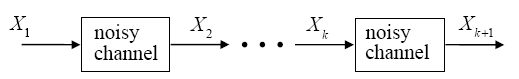
\includegraphics[width=0.6\linewidth]{HWs//HW2//figures/2.png}
\end{figure}
\begin{align*}
    P(X_{k+1} = 0 | X_k = 0) = 0.6, P(X_{k+1} = 1 | X_k = 0) = 0.4 \\
    P(X_{k+1} = 0 | X_k = 1) = 0.3, P(X_{k+1} = 1 | X_k = 1) = 0.7
\end{align*}
}
\begin{enumerate}
    \item[(a)] Find $P(X_2 = 1)$.
    \myAnswer{
    \begin{align*}
        P(X_2 = 1) &= P(X_2 = 1 | X_1 = 0) \cdot P(X_1 = 0) + P(X_2 = 1 | X_1 = 1) \cdot P(X_1 = 1) \\
        &= 0.4 \times 0.2 + 0.7 \times 0.8 = \underline{0.64}
    \end{align*}
    }
    \item[(b)] Find $P(X_3 = 1)$. 
    \myAnswer{
    \begin{align*}
        P(X_3 = 1) &= P(X_3 = 1 | X_2 = 0) \cdot P(X_2 = 0) + P(X_3 = 1 | X_2 = 1) \cdot P(X_2 = 1) \\
        &= 0.4 \times (1 - 0.64) + 0.7 \times 0.64 = \underline{0.592}
    \end{align*}
    }
    \item[(c)] Find $P(X_1 = 0 | X_3 = 1)$. 
    \myAnswer{
    \begin{align*}
        P(X_1 = 0 | X_3 = 1) &= \frac{P(X_3 = 1 | X_1 = 0) \cdot P(X_1 = 0)}{P(X_3 = 1)} \\
        &= \frac{\sum_{i=0,1}(P(X_3 = 1 | X_2 = i) \cdot P(X_2 = i | X_1 = 0)) \cdot P(X_1 = 0)}{P(X_3 = 1)} \\
        &= \frac{(0.4\times 0.6 + 0.7\times 0.4) \times 0.2}{0.592} \approx \underline{0.223}
    \end{align*}
    }
    \item[(d)] Find $\lim_{n\rightarrow \infty} P(X_n = 0)$. \\
    \myAnswer{
    When $n\rightarrow \infty$, $P(X_n = 0) = P(X_{n-1} = 0)$. \\ Let $P(X_n = 0) = P(X_{n-1} = 0) = x$, we have
    \begin{align*}
        P(X_n = 0) &= P(X_n = 0 | X_{n-1} = 0) \cdot P(X_{n-1} = 0) + P(X_n = 0 | X_{n-1} = 1) \cdot P(X_{n-1} = 1) \\ 
        &= 0.6 x + 0.3 (1 - x) = x \Rightarrow x = 3/7 \approx \underline{0.4286}
    \end{align*}
    }
\end{enumerate}
